\documentclass[11pt]{article}

\usepackage[margin=1in]{geometry}
\usepackage{amsmath,amssymb}
\usepackage{booktabs}
\usepackage{array}
\usepackage{tabularx}
\usepackage{graphicx}
\usepackage{float}
\usepackage{microtype}
\usepackage[round,authoryear]{natbib}
\usepackage[hidelinks]{hyperref}
\usepackage{caption}
\usepackage{enumitem}

\graphicspath{{figures/}}
\setlength{\parindent}{0pt}
\setlength{\parskip}{0.55em}
\setlength{\emergencystretch}{2em}
\captionsetup{font=small,labelfont=bf}

\newcommand{\BH}{Buy\&Hold}
\newcommand{\JM}{JM}
\newcommand{\HMM}{HMM}
\newcommand{\ind}{\mathbf{1}}

\title{\textbf{One Risk Measure, Fewer Trades:}\\
A Parsimonious Jump Model for U.S. Downside Protection}
\author{Tan Le}
\date{July 2026}

\begin{document}
\maketitle

\begin{abstract}
Regime models are useful only if their signals survive the delay between observing the market and trading it. We revisit the market-or-cash experiment of \citet{shu2024}, using public equity and cash-rate proxies, past information only, monthly walk-forward model selection, a one-day trading delay, and 10 basis points of one-way trading cost. The public-proxy reconstruction does not recover the original three-market ordering: the standard three-feature statistical jump model does not beat both a Gaussian hidden Markov model and buy-and-hold in the United States, Germany, or Japan. A simpler model does much better in the United States. Using exponentially weighted downside deviation as the only jump-model feature raises net Sharpe from 0.570 to 0.908, improves maximum drawdown from -33.9\% to -19.4\%, and reduces position changes from 21 to 11. Its drawdown is essentially the same as the HMM's, but it trades far less and earns a higher Sharpe ratio. A prespecified control that triples the downside-deviation loss retains most of the improvement, suggesting that feature content matters more than loss scale alone. The same model does not beat buy-and-hold in Germany or Japan, and one-state fits remain common there. The evidence therefore supports a focused U.S. hypothesis about feature parsimony, not a cross-market or live-performance claim.
\end{abstract}

\noindent\textbf{Keywords:} statistical jump models; market regimes; downside deviation; feature parsimony; hidden Markov models; downside risk.

\section{Introduction}

A market-regime signal has to solve a practical problem before it solves a statistical one. A signal that changes every few days is difficult to trade and quickly loses money to delay and transaction costs. A signal that almost never changes is easier to trade, but may react too late to protect a portfolio. The useful signal lies somewhere between those extremes.

The 0/1 strategy makes this trade-off easy to see. It holds the equity market when the current regime is favorable and local cash when it is unfavorable. There is no portfolio optimizer to conceal a weak signal. If the regime model reacts to noise, the strategy whipsaws. If it reacts too slowly, the strategy stays invested through the drawdown or misses the rebound.

\citet{shu2024} use this setting to compare a Gaussian hidden Markov model (HMM) with a statistical jump model (JM). The HMM estimates a latent Markov chain from returns. The JM is closer to temporal clustering: it assigns observations to fitted centers and charges a fixed cost whenever the state changes \citep{bemporad2018,nystrup2020}. Shu, Yu, and Mulvey select the HMM smoothing window and JM jump penalty with a trailing eight-year validation exercise that includes trading delay and transaction cost. On their licensed 1990--2023 data, the JM-guided strategy has a higher Sharpe ratio and a smaller maximum drawdown than both the HMM strategy and buy-and-hold in the United States, Germany, and Japan.

We reconstruct the same economic question on public proxies. The reconstruction preserves the parts of the design that matter for a live strategy: models use past data only, tuning is walk-forward, a signal formed after day $t$ is first reflected in portfolio return at $t+2$, and every one-way position change costs 10 basis points. It is not a numerical replication. The public instruments, cash-rate definitions, warm-up histories, and evaluation periods differ materially from the licensed sample.

The standard three-feature JM does not recover the original model ordering on these proxies. This failure leads to a smaller question: does the model need all three features? Shu et al. use one downside-risk measure---exponentially weighted downside deviation---and two exponentially weighted Sortino ratios. The return features are economically sensible, but they are also noisy. Removing them produces a one-dimensional JM whose state changes are driven only by recent downside risk.

That simple model is the clearest empirical result in the project. In the U.S. proxy sample, the downside-deviation-only JM achieves a net Sharpe ratio of 0.908, compared with 0.570 for the standard JM, 0.654 for the HMM, and 0.513 for buy-and-hold. It also cuts the standard JM's maximum drawdown from -33.9\% to -19.4\% and reduces the number of position changes from 21 to 11. The result is not reproduced in Germany or Japan.

A one-feature loss is smaller, in raw objective units, than a three-feature loss. Keeping the same jump-penalty grid could therefore make the one-feature model look more persistent for a mechanical reason. We address that concern with a prespecified scale control that multiplies the downside-deviation loss by three while leaving the data, grid, timing, refits, and validation procedure unchanged. The control keeps most of the improvement over the standard JM. This does not prove that the Sortino features are harmful, but it makes raw loss scale an incomplete explanation.

The paper makes three contributions. First, it provides a transparent public-proxy reconstruction of the economic test in \citet{shu2024}. Second, it shows that a one-feature downside-risk JM can deliver a much cleaner U.S. market-or-cash path than the standard three-feature model. Third, it separates feature removal from a simple loss-scale effect and reports the cases where the interpretation breaks down. The evidence is deliberately narrow: it is exploratory, the through-2023 sample has been inspected repeatedly, and no untouched confirmation period is used.

\section{Data and empirical design}

\subsection{Public proxies and evaluation samples}

The parent study uses licensed total-return indices and country-specific three-month Treasury-bill yields beginning in 1970. Those exact series and the complete empirical package are not available. We therefore use public instruments that play similar economic roles, summarized in Table~\ref{tab:data}. The data are capped at 31 December 2023.

\begin{table}[H]
\centering
\caption{Public proxy data and primary evaluation samples.}
\label{tab:data}
\small
\begin{tabularx}{\textwidth}{l X X l l}
\toprule
Market & Equity proxy & Cash-rate proxy & Evaluation start & Observations \\
\midrule
US & S\&P 500 total-return candidate (Yahoo \texttt{\char94 SP500TR}) & Three-month U.S. Treasury-bill discount rate (FRED \texttt{DTB3}) & 4 Dec 2007 & 4,046 \\
Germany & DAX performance-index candidate (Yahoo \texttt{\char94 GDAXI}) & Monthly three-month interbank-rate proxy (FRED \texttt{IR3TIB01DEM156N}) & 3 Jan 2008 & 4,059 \\
Japan & Nikkei 225 price index (Yahoo \texttt{\char94 N225}) & Monthly uncollateralized call-rate proxy (Bank of Japan \texttt{STRACLUC3M}) & 7 May 2009 & 3,586 \\
\bottomrule
\end{tabularx}
\begin{minipage}{0.96\textwidth}
\footnotesize\emph{Notes:} All samples end on 29 December 2023 after training, validation, trading-delay, and common-date alignment. The Japanese equity proxy excludes dividends. The German and Japanese cash series are not Treasury-bill series. These differences prevent a like-for-like replication of the parent sample.
\end{minipage}
\end{table}

Equity simple return is computed from consecutive valid market dates. Cash rates are converted to daily returns and aligned backward only after a conservative publication lag. No missing value is filled from the future. Excess return is equity return minus the aligned cash return.

The original JM features are based on excess return and follow the downside-risk tradition of \citet{roy1952} and \citet{markowitz1959}. They are exponentially weighted downside deviation with half-life 10 and Sortino ratios with half-lives 20 and 60:
\begin{equation}
DD_h(t)=\sqrt{\operatorname{EWM}_h\!\left[(r_t^x)^2\ind\{r_t^x<0\}\right]},
\qquad
Sortino_h(t)=\frac{\operatorname{EWM}_h[r_t^x]}{DD_h(t)}.
\end{equation}
Features are standardized on the training window only.

\subsection{The market-or-cash strategy}

Let $a_t\in\{0,1\}$ denote the equity signal formed after observing day $t$. The strategy holds equity when $a_t=1$ and cash when $a_t=0$. Following \citet{shu2024}, the signal is executed at the close of the next trading day. The first affected return is therefore day $t+2$.

If $w_u$ is the equity position earning the return on day $u$, the net portfolio return is
\begin{equation}
r^{p,net}_u=w_u r^e_u+(1-w_u)r^c_u-0.001\lvert w_u-w_{u-1}\rvert.
\end{equation}
The first observed position receives no artificial opening cost. Annualized Sharpe is computed from daily net excess return, maximum drawdown includes initial wealth one, and turnover is
\begin{equation}
Turnover=\frac{1}{2}\,252\,\operatorname{mean}\lvert w_u-w_{u-1}\rvert.
\end{equation}
The factor one-half counts an equity-to-cash-to-equity round trip once.

\subsection{Models and walk-forward selection}

The benchmark HMM is a two-state Gaussian model fitted to daily log return on a trailing 3,000-observation window. The lower-volatility state is treated as favorable. The terminal Viterbi state is smoothed by a trailing majority rule, with the smoothing window selected monthly.

The standard two-state JM is fitted on the three standardized features $x_t\in\mathbb{R}^3$ by minimizing
\begin{equation}
\min_{\Theta,S}\sum_{t=0}^{T-1}\frac{1}{2}\lVert x_t-\theta_{s_t}\rVert_2^2
+\lambda\sum_{t=1}^{T-1}\ind\{s_t\neq s_{t-1}\}.
\label{eq:fixedjm}
\end{equation}
The model is refitted in January and July on the trailing 3,000 complete observations. The state with the higher cumulative training excess return is labeled favorable. Between refits, the scaler and centers are frozen and only the terminal state of the exact dynamic-programming path is emitted.

For both HMM and JM, the smoothing parameter is selected at the end of each month by replaying the preceding eight calendar years. Candidate signals are evaluated with the same trading delay and transaction cost as the outer strategy. The candidate with the highest validation Sharpe is used during the following month, again subject to the trading delay. This follows the practical selection principle in \citet{shu2024}: tune the regime signal for the economic task in which it will be used.

\subsection{The parsimonious model and its scale control}

The downside-deviation-only model replaces the three-dimensional observation in Equation~\eqref{eq:fixedjm} with standardized downside deviation $z_t^{DD}$:
\begin{equation}
\min_{\theta,S}\sum_{t=0}^{T-1}\frac{1}{2}(z_t^{DD}-\theta_{s_t})^2
+\lambda\sum_{t=1}^{T-1}\ind\{s_t\neq s_{t-1}\}.
\label{eq:dd}
\end{equation}
Everything else---the complete-row calendar, training window, refit schedule, jump-penalty grid, validation window, signal timing, and trading cost---is unchanged.

This comparison has an immediate scale confound. Equation~\eqref{eq:dd} has one standardized loss coordinate, whereas the standard JM has three. We therefore also estimate a three-times-loss control:
\begin{equation}
J_3(\theta,S;\lambda)=\sum_{t=0}^{T-1}\frac{3}{2}(z_t^{DD}-\theta_{s_t})^2
+\lambda\sum_{t=1}^{T-1}\ind\{s_t\neq s_{t-1}\}.
\label{eq:scaled}
\end{equation}
For the same data and tie rules,
\begin{equation}
J_3(\theta,S;\lambda)=3J_1(\theta,S;\lambda/3),
\end{equation}
so the control has a precise mechanical interpretation. The raw candidate grid is deliberately left unchanged; the exercise asks whether the observed result disappears when the observation loss is returned to roughly the three-coordinate scale.

The DD-only model was one member of a frozen five-model challenger suite, not the only idea examined. The other challengers fixed $\lambda=50$, required two consecutive observations before switching, added matured future-return information to the training loss without using it online, or replaced squared Euclidean loss with cityblock loss. Their complete results are reported in Appendix~\ref{app:suite}.

\section{Results}

\subsection{The public proxy does not reproduce the parent ordering}

Table~\ref{tab:parentproxy} compares the headline Sharpe ratios reported by \citet{shu2024} with the public-proxy reconstruction. The numbers are not like-for-like: the source instruments and test periods differ. The comparison is useful because it shows the empirical problem that motivates the parsimonious model. On the public proxies, the standard JM is not the strongest of buy-and-hold, HMM, and JM in any market.

\begin{table}[H]
\centering
\caption{Net Sharpe in the parent study and the public-proxy reconstruction.}
\label{tab:parentproxy}
\begin{tabular}{lcc}
\toprule
Market & Shu et al.: \BH{}/HMM/JM & Public proxy: \BH{}/HMM/standard JM \\
\midrule
US & 0.48 / 0.54 / 0.68 & 0.513 / 0.654 / 0.570 \\
Germany & 0.30 / 0.35 / 0.44 & 0.290 / 0.008 / 0.166 \\
Japan & 0.12 / 0.19 / 0.31 & 0.545 / 0.399 / 0.329 \\
\bottomrule
\end{tabular}
\end{table}

This should be read as a proxy non-replication, not as a refutation of the original study. The Japanese sample makes the difference especially clear: public-proxy buy-and-hold Sharpe is about 0.545, compared with 0.12 in the parent paper, and the proxy excludes dividends.

\subsection{One risk measure changes the U.S. result}

Table~\ref{tab:mainresults} reports the main net results. The U.S. DD-only JM is the only tested variant that beats both same-sample controls. Its Sharpe ratio is 0.908, a gain of 0.338 over the standard JM and 0.254 over the stronger benchmark, the HMM.

\begin{table}[H]
\centering
\caption{Primary-delay net results. MDD, turnover, and cash are percentages.}
\label{tab:mainresults}
\small
\resizebox{\textwidth}{!}{%
\begin{tabular}{llrrrrr}
\toprule
Market & Model & Sharpe & MDD & Turnover & Cash fraction & Switches \\
\midrule
US & \BH{} & 0.512964 & -53.963 & 0.000 & 0.000 & 0 \\
US & Gaussian HMM & 0.653725 & -19.363 & 143.253 & 24.221 & 46 \\
US & Standard three-feature JM & 0.569865 & -33.857 & 65.398 & 21.157 & 21 \\
US & DD-only JM & \textbf{0.907547} & \textbf{-19.364} & \textbf{34.256} & 13.569 & \textbf{11} \\
US & Three-times DD JM & 0.884130 & -19.531 & 46.713 & 14.137 & 15 \\
\addlinespace
Germany & \BH{} & 0.289638 & -53.876 & 0.000 & 0.000 & 0 \\
Germany & Gaussian HMM & 0.007599 & -54.590 & 105.543 & 11.949 & 34 \\
Germany & Standard three-feature JM & 0.166440 & -38.779 & 99.335 & 18.280 & 32 \\
Germany & DD-only JM & 0.226442 & -42.833 & 80.710 & 11.358 & 26 \\
Germany & Three-times DD JM & 0.195916 & -44.517 & 49.667 & 11.210 & 16 \\
\addlinespace
Japan & \BH{} & 0.544589 & -31.799 & 0.000 & 0.000 & 0 \\
Japan & Gaussian HMM & 0.398539 & -34.656 & 130.006 & 5.633 & 37 \\
Japan & Standard three-feature JM & 0.329270 & -32.162 & 45.678 & 27.886 & 13 \\
Japan & DD-only JM & 0.423891 & -43.241 & 66.760 & 8.728 & 19 \\
Japan & Three-times DD JM & 0.428050 & -34.529 & 80.814 & 13.887 & 23 \\
\bottomrule
\end{tabular}}
\end{table}

The U.S. risk and activity profile is as important as the Sharpe ratio. DD-only improves maximum drawdown from -33.9\% for the standard JM to -19.4\%, essentially matching the HMM's -19.4\%. It does so with turnover of 34.3\%, compared with 143.3\% for the HMM, and with 11 position changes instead of 46. The model spends only 13.6\% of the sample in cash, compared with 24.2\% for the HMM.

Figure~\ref{fig:uspaths} shows the difference directly. The standard JM and HMM identify many more cash intervals. The DD-only path keeps the long 2008--2009 defensive episode, avoids a portion of the 2020 crash, and exits during the 2022 decline, but removes several shorter switches that do not improve the net strategy.

\begin{figure}[H]
\centering
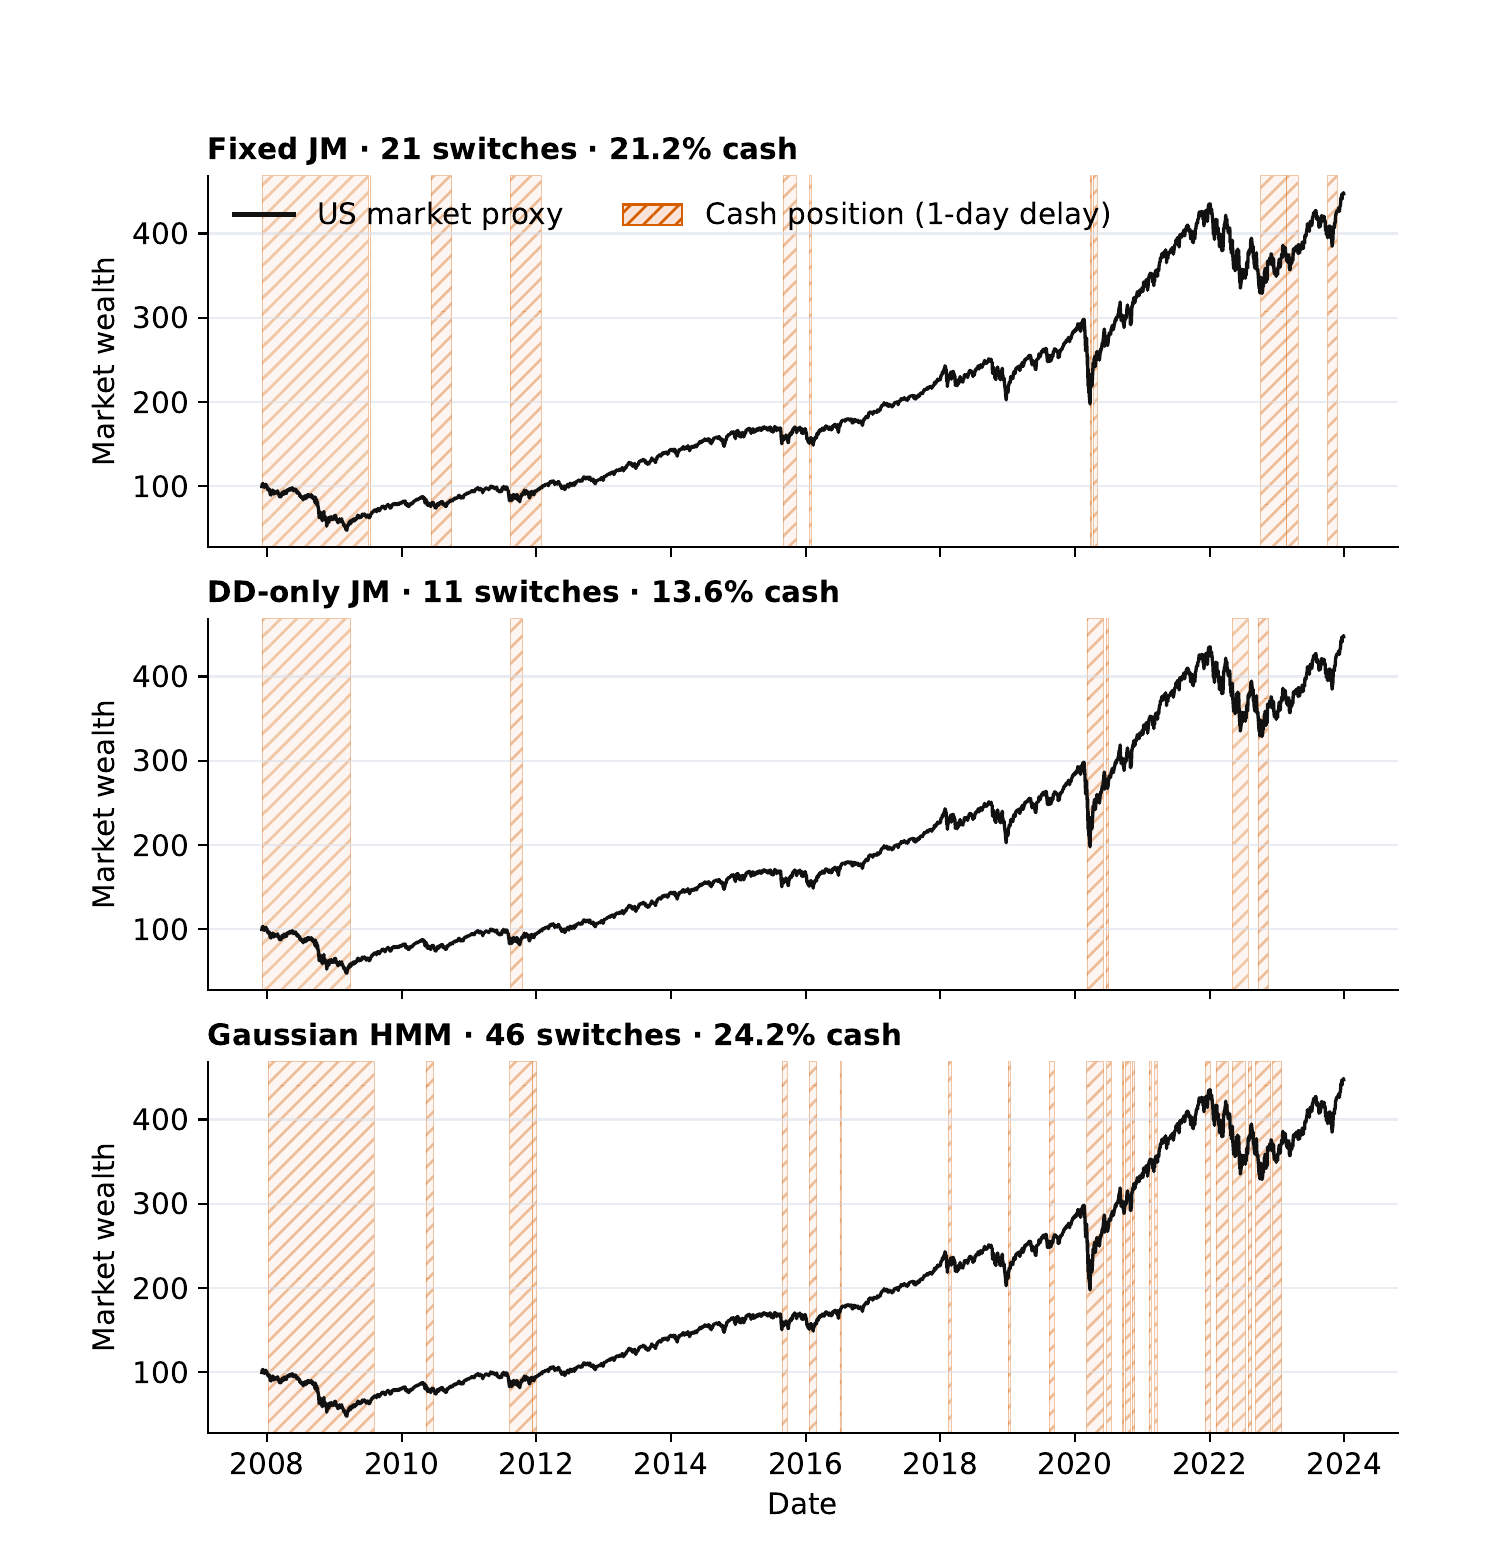
\includegraphics[width=0.94\textwidth]{fig_us_paths.png}
\caption{U.S. market wealth and delayed cash positions, 4 December 2007 to 29 December 2023. Shading is the executable cash position after the one-day trading delay, not a latent ground-truth label.}
\label{fig:uspaths}
\end{figure}

\subsection{The result is local, not cross-market}

The same DD-only specification raises the standard JM Sharpe in all three markets: by 0.338 in the United States, 0.060 in Germany, and 0.095 in Japan. That comparison alone is not enough. The relevant economic question is whether the model also beats the stronger of buy-and-hold and HMM on the same dates.

It does so only in the United States. In Germany, DD-only remains below buy-and-hold and has a worse maximum drawdown than the standard JM. In Japan, it remains well below buy-and-hold, its maximum drawdown deteriorates to -43.2\%, and its switch count rises from 13 to 19. Figure~\ref{fig:wealth} makes the asymmetry visible: DD-only finishes well above the other strategies in the U.S. panel, but not in the German or Japanese panels.

\begin{figure}[H]
\centering
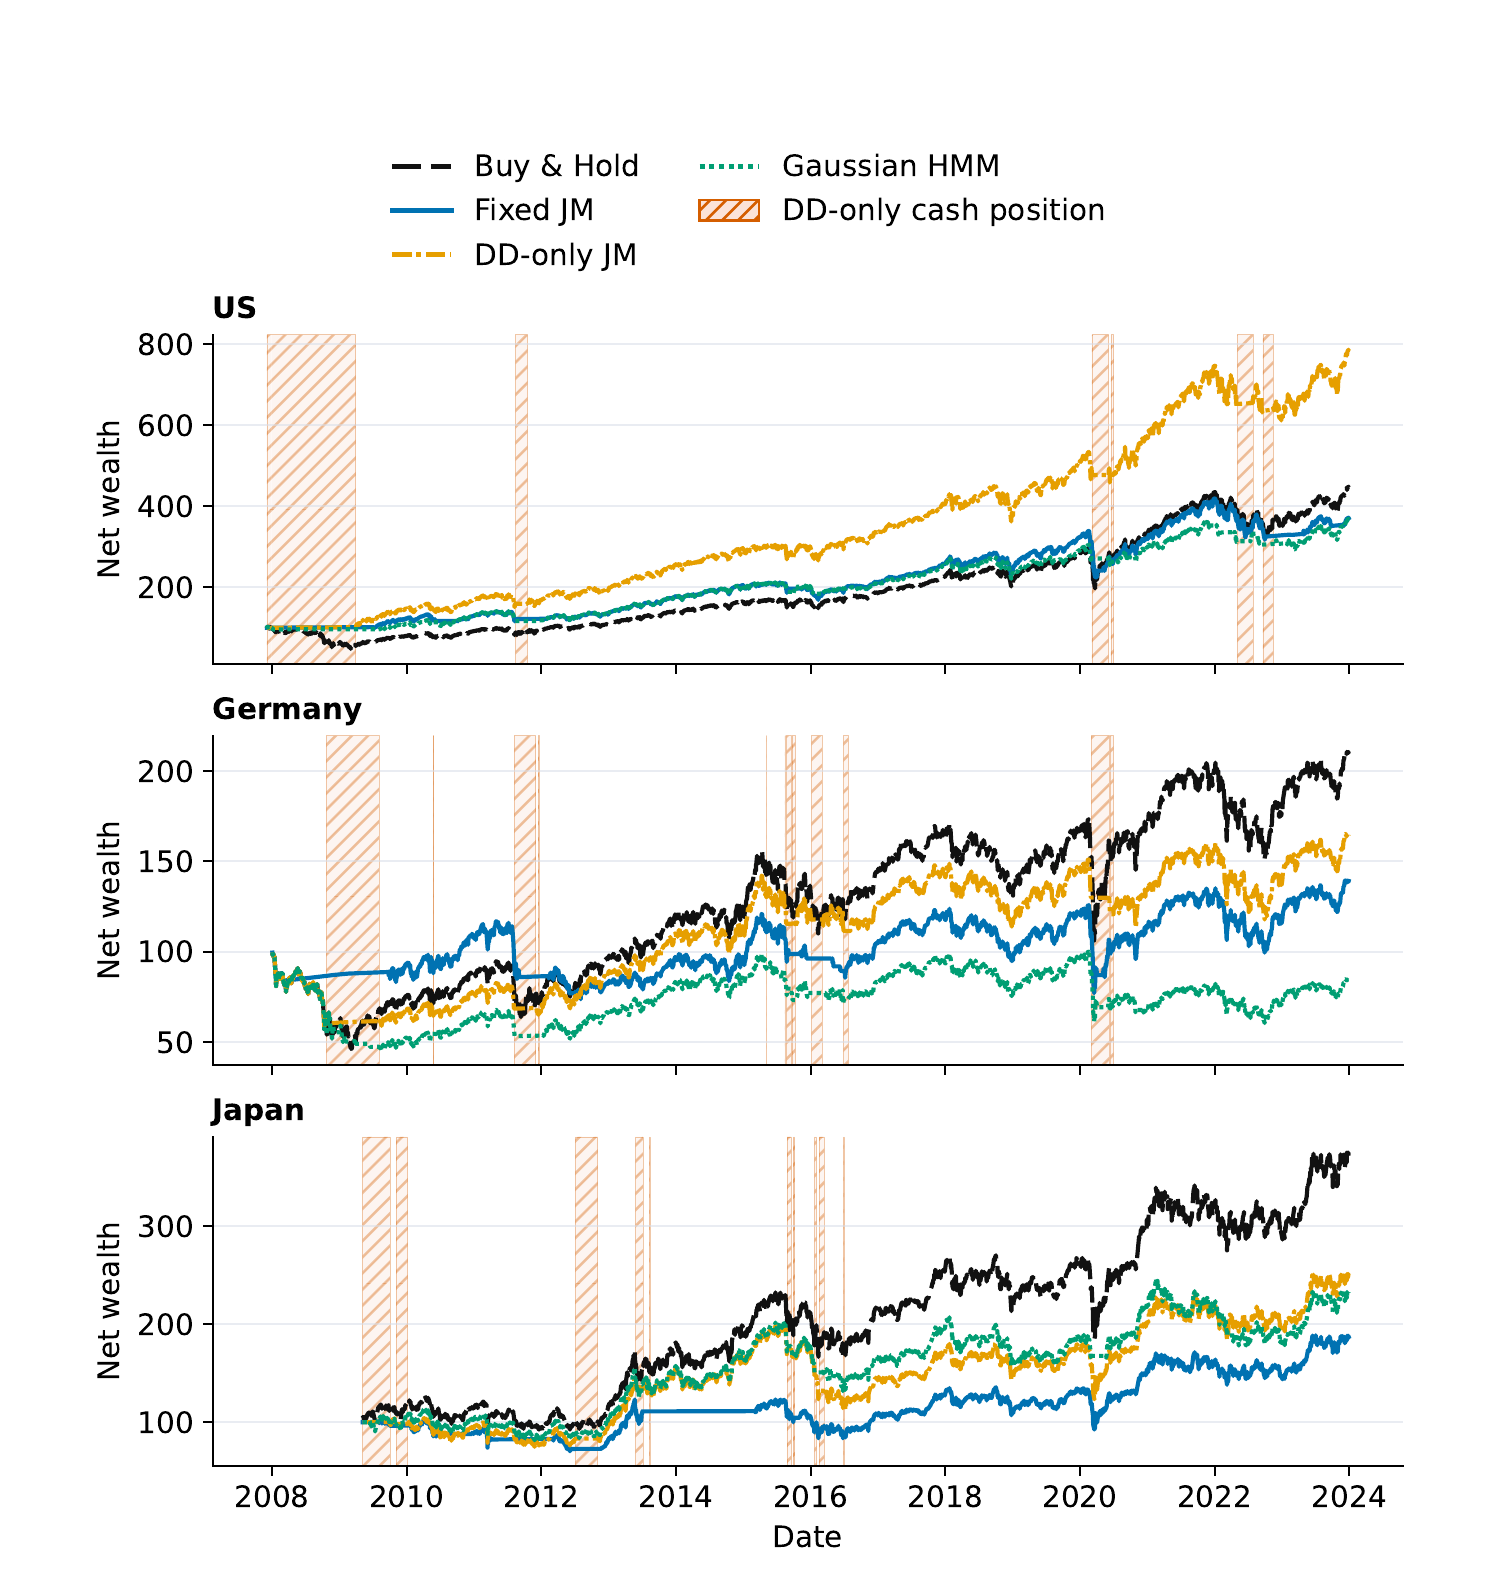
\includegraphics[width=0.94\textwidth]{fig_wealth_markets.png}
\caption{Net executable wealth after 10-basis-point one-way costs. The hatching marks the delayed DD-only cash position. DD-only finishes above both buy-and-hold and HMM in the United States, but not in Germany or Japan.}
\label{fig:wealth}
\end{figure}

These external-market failures are part of the result. Choosing DD-only for the United States, a lagged adaptive model for Germany, and another model for Japan after observing all outcomes would create an ex-post envelope, not a deployable rule.

\subsection{The scale control keeps most of the improvement}

Multiplying the DD loss by three changes the monthly penalty choices in the expected direction. Relative to ordinary DD-only, the selector chooses a larger raw $\lambda$ in 73.7\%, 81.3\%, and 66.1\% of paired U.S., German, and Japanese months. The resulting state paths do not move uniformly: the control adds four switches in the United States, removes ten in Germany, and adds four in Japan.

The Sharpe ratio changes only modestly. Scaled minus ordinary DD-only is -0.023 in the United States, -0.031 in Germany, and +0.004 in Japan. More importantly, scaled DD still exceeds the standard JM Sharpe by 0.314, 0.029, and 0.099 across the three markets. Most of the one-feature improvement therefore survives the scale adjustment.

\begin{figure}[H]
\centering
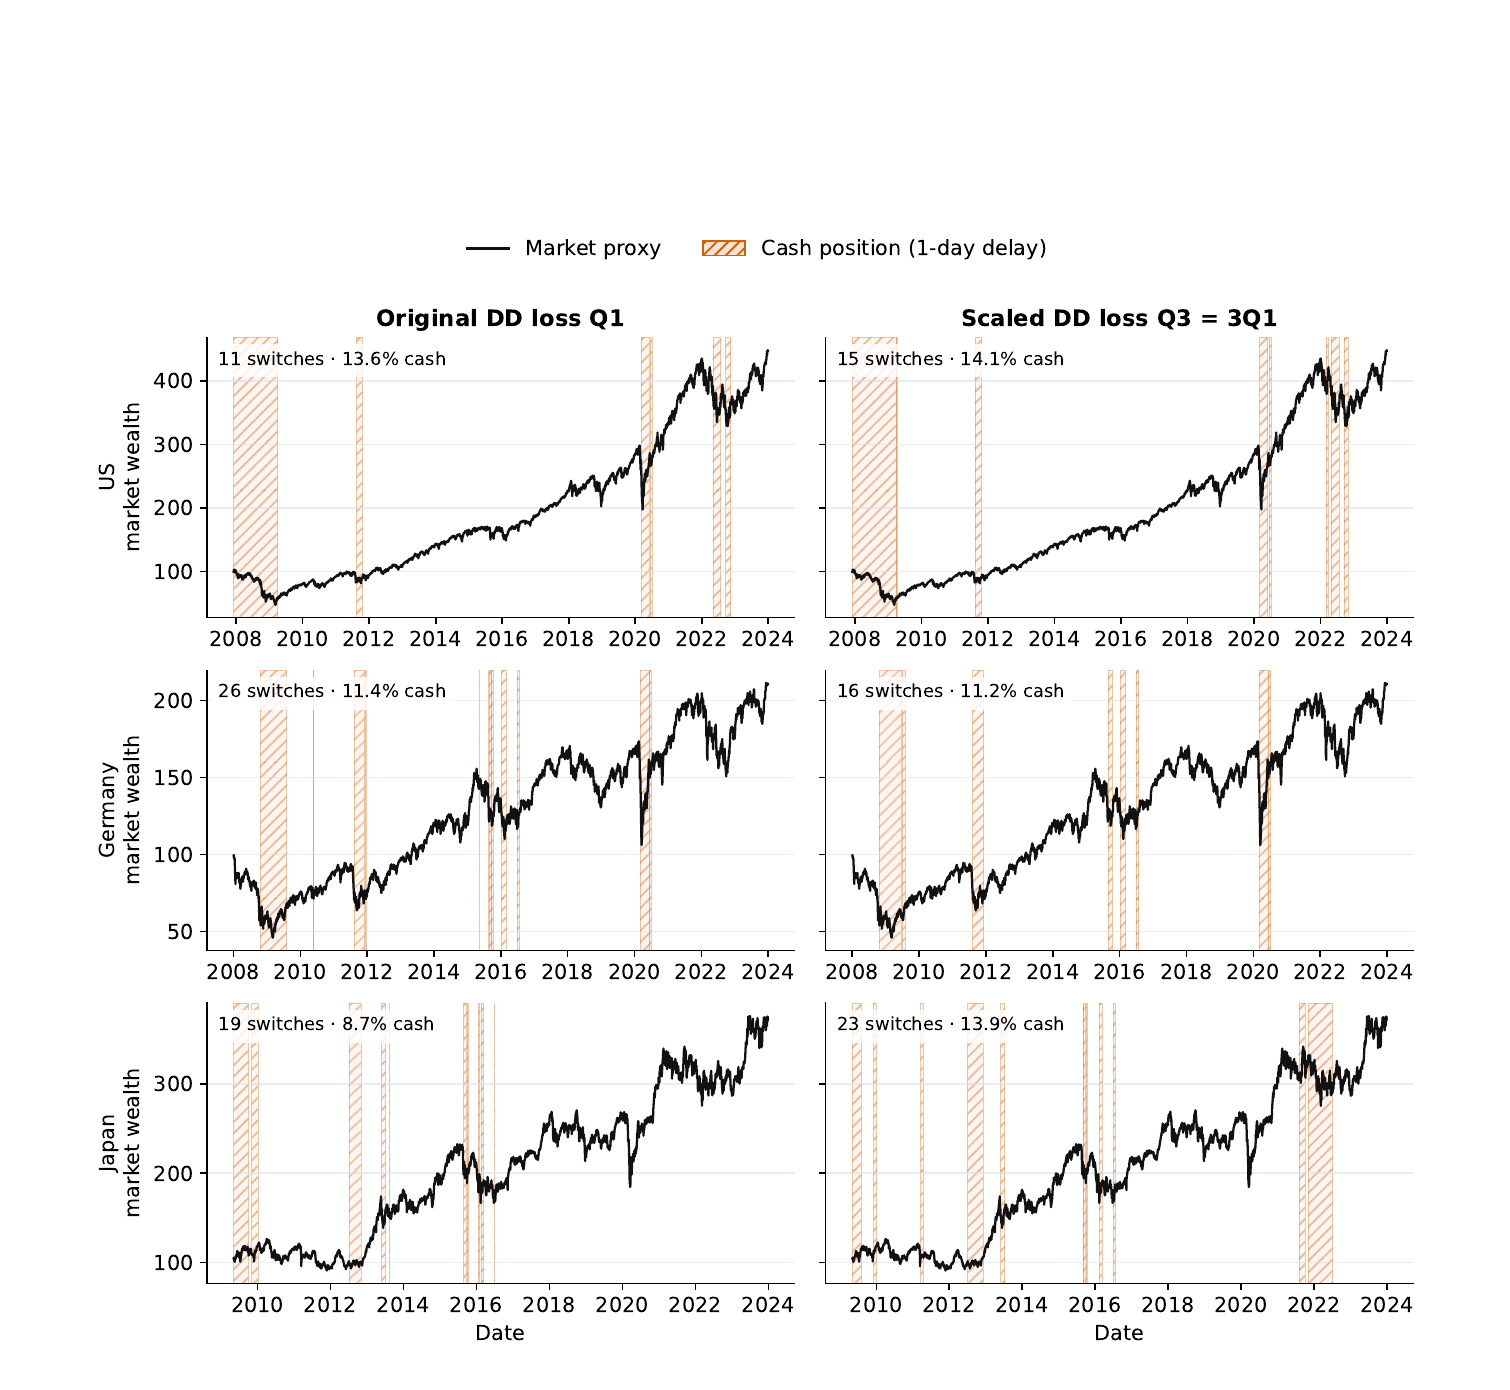
\includegraphics[width=0.94\textwidth]{fig_dd_scale_paths.png}
\caption{Ordinary and three-times-DD delayed cash positions on identical dates. Scaling the observation loss makes the German path calmer but makes the U.S. and Japanese paths more active.}
\label{fig:scale}
\end{figure}

The control supports a limited interpretation. The U.S. improvement is unlikely to be explained mainly by the one-dimensional loss being smaller relative to the unchanged penalty grid. It does not establish that the two Sortino features are universally harmful. The finite grid still binds in Germany and Japan, and the one-dimensional model often collapses to a single fitted state there.

\subsection{Degenerate fits and repeated inspection}

A two-state algorithm can return a training fit that occupies only one state. The decoder remains deterministic---the unused state is made unreachable---but the selected candidate is then economically a one-state rule, not evidence that two regimes were recovered.

For ordinary DD-only, monthly validation selected a collapsed fit in 0 of 194 U.S. months, 43 of 193 German months, and 75 of 177 Japanese months. For three-times DD, the corresponding counts were 0, 44, and 63. The U.S. result is therefore not driven by selected one-state fits. In Germany and Japan, collapse is material and weakens any regime interpretation.

The data through 2023 have also been used repeatedly during model development. The five-model challenger suite and the scale control were frozen before their respective results, but the broader U.S., German, and Japanese samples are not untouched holdouts. The correct interpretation is exploratory development evidence. A performance claim would require a fixed specification evaluated on data that did not shape it.

\section{Discussion}

The U.S. result suggests a simple possibility: recent downside risk may contain most of the information that this market-or-cash JM can use reliably, while the two smoothed Sortino coordinates add more estimation noise than economic value on this sample. This interpretation is plausible because return averages are much noisier than risk measures at daily frequency, even after exponential smoothing.

There is also a model-selection explanation. The jump penalty is selected from a finite raw grid. Changing the feature set changes the scale and geometry of the observation loss, which changes which penalties are effective and which state paths are reachable. The three-times-loss control shows that raw scale is not the whole story, but it does not isolate a unique causal channel. The result may reflect a combination of cleaner feature content, simpler clustering geometry, and more favorable interaction with the finite validation grid.

The cross-market evidence prevents a stronger claim. Germany and Japan have different proxy definitions, different cash-rate frequencies, and different market paths. The Japanese price-index proxy excludes dividends and has a buy-and-hold Sharpe far above the parent paper's sample. A model that protects the U.S. market during a few long drawdowns may miss too many rapid recoveries elsewhere.

The most useful next test is therefore not another search over the same through-2023 data. It is a genuinely fixed, prospective evaluation of the DD-only and three-times-DD specifications. The present result gives that test a clear target: preserve the U.S. reduction in drawdown and trading activity without relying on market-specific retuning after outcomes are known.

\section{Conclusion}

\citet{shu2024} show that a persistent regime signal can be evaluated in the same terms in which it would be traded: with delayed decisions, transaction costs, and an explicit market-or-cash allocation. Our public-proxy reconstruction preserves that economic discipline but does not reproduce the original three-market ranking.

The strongest result comes from making the JM smaller, not more elaborate. A model driven only by exponentially weighted downside deviation produces a much better U.S. strategy than the standard three-feature JM. It earns a higher net Sharpe ratio than both buy-and-hold and the Gaussian HMM, matches the HMM's maximum drawdown, and trades far less. A scale-matched control retains most of the gain, making feature removal a more convincing explanation than raw loss scale alone.

The same rule does not win in Germany or Japan, and degenerate one-state fits are frequent in those markets. The evidence therefore supports a focused hypothesis: for U.S. downside protection, one carefully chosen risk feature may be more useful than a small mixed set of risk and return features. It does not yet support a general performance claim.

\appendix

\section{The full simple-challenger suite}
\label{app:suite}

Table~\ref{tab:suite} reports all five frozen challengers. A positive benchmark gap means the model's Sharpe exceeds both same-sample buy-and-hold and HMM. DD-only is the only challenger with a positive gap in any market, and that occurs only in the United States.

\begin{table}[H]
\centering
\caption{Net Sharpe and gap to the stronger same-sample control.}
\label{tab:suite}
\small
\begin{tabular}{llrr}
\toprule
Market & Challenger & Sharpe & Benchmark gap \\
\midrule
US & Static $\lambda=50$ & 0.586183 & -0.067542 \\
US & DD-only & 0.907547 & +0.253822 \\
US & Two-observation confirmation & 0.619291 & -0.034433 \\
US & Return-aware training loss & 0.559865 & -0.093860 \\
US & Robust $L_1$ loss & 0.372797 & -0.280928 \\
\addlinespace
Germany & Static $\lambda=50$ & 0.156219 & -0.133419 \\
Germany & DD-only & 0.226442 & -0.063196 \\
Germany & Two-observation confirmation & 0.149925 & -0.139713 \\
Germany & Return-aware training loss & 0.149742 & -0.139896 \\
Germany & Robust $L_1$ loss & 0.173382 & -0.116256 \\
\addlinespace
Japan & Static $\lambda=50$ & 0.183934 & -0.360656 \\
Japan & DD-only & 0.423891 & -0.120698 \\
Japan & Two-observation confirmation & 0.297227 & -0.247362 \\
Japan & Return-aware training loss & 0.329270 & -0.215320 \\
Japan & Robust $L_1$ loss & 0.361360 & -0.183230 \\
\bottomrule
\end{tabular}
\end{table}

Confirmation removes one-observation excursions and reduces switching in the United States and Germany, but it does not beat the stronger benchmark. The return-aware loss changes very few selected signal dates and produces no Sharpe improvement. Robust $L_1$ loss changes paths materially but raises activity in the United States and Japan.

\section{Reproducibility note}

The accepted pipeline stores frozen study contracts, exact model and accounting outputs, source inventories, and independent replay checks. The primary sample is hard-capped at 31 December 2023. The verification routines check the one-day trading delay, $t+2$ return and cost accounting, 10-basis-point one-way costs, the paper turnover convention, monthly selection, candidate paths, and reported metrics. These controls establish numerical agreement for the retained experiments; they do not turn an inspected development sample into a confirmatory holdout.

\begin{thebibliography}{99}

\bibitem[Bemporad et~al.(2018)Bemporad, Breschi, Piga, and Boyd]{bemporad2018}
Bemporad, A., Breschi, V., Piga, D., and Boyd, S.~P. (2018).
Fitting jump models.
\emph{Automatica}, 96, 11--21.

\bibitem[Bulla et~al.(2011)Bulla, Mergner, Bulla, Sesbo\"ue, and Chesneau]{bulla2011}
Bulla, J., Mergner, S., Bulla, I., Sesbo\"ue, A., and Chesneau, C. (2011).
Markov-switching asset allocation: Do profitable strategies exist?
\emph{Journal of Asset Management}, 12, 310--321.

\bibitem[Markowitz(1959)]{markowitz1959}
Markowitz, H. (1959).
\emph{Portfolio Selection}.
Yale University Press.

\bibitem[Nystrup et~al.(2020)Nystrup, Lindstr\"om, and Madsen]{nystrup2020}
Nystrup, P., Lindstr\"om, E., and Madsen, H. (2020).
Learning hidden Markov models with persistent states by penalizing jumps.
\emph{Expert Systems with Applications}, 150, 113307.

\bibitem[Nystrup et~al.(2021)Nystrup, Kolm, and Lindstr\"om]{nystrup2021}
Nystrup, P., Kolm, P.~N., and Lindstr\"om, E. (2021).
Feature selection in jump models.
\emph{Expert Systems with Applications}, 184, 115558.

\bibitem[Pagan and Sossounov(2003)]{pagan2003}
Pagan, A.~R. and Sossounov, K.~A. (2003).
A simple framework for analysing bull and bear markets.
\emph{Journal of Applied Econometrics}, 18(1), 23--46.

\bibitem[Roy(1952)]{roy1952}
Roy, A.~D. (1952).
Safety first and the holding of assets.
\emph{Econometrica}, 20(3), 431--449.

\bibitem[Schwert(1989)]{schwert1989}
Schwert, G.~W. (1989).
Why does stock market volatility change over time?
\emph{Journal of Finance}, 44(5), 1115--1153.

\bibitem[Shu et~al.(2024)Shu, Yu, and Mulvey]{shu2024}
Shu, Y., Yu, C., and Mulvey, J.~M. (2024).
Downside risk reduction using regime-switching signals: A statistical jump model approach.
\emph{Journal of Asset Management}, 25, 493--507.

\end{thebibliography}

\end{document}
